\documentclass[handout,aspectratio=1610]{beamer}
%\documentclass[aspectratio=1610]{beamer}

%\usepackage[T1]{fontenc}
\usepackage[ngerman]{babel}
\usepackage{color}
\usepackage{colortbl}
\usepackage{textcomp}
\usepackage{multirow}
\usepackage{nicefrac}
\usepackage{multicol}
\usepackage{gb4e-}
\usepackage{verbatim}
\usepackage{cancel}
\usepackage{graphicx}
\usepackage{hyperref}
\usepackage{verbatim}
\usepackage{boxedminipage}
\usepackage{rotating}
\usepackage{booktabs}
\usepackage{bbding}
\usepackage{soul}

\usepackage{tikz}
\usetikzlibrary{positioning,arrows,cd}
\tikzset{>=latex}

\usepackage[linguistics]{forest}

\usepackage{FiraSans}

\usepackage[maxbibnames=99,
  maxcitenames=2,
  uniquelist=false,
  backend=biber,
  doi=false,
  url=false,
  isbn=false,
  bibstyle=biblatex-sp-unified,
  citestyle=sp-authoryear-comp]{biblatex}
\addbibresource{rs}

\forestset{
  Ephr/.style={draw, ellipse, thick, inner sep=2pt},
  Eobl/.style={draw, rounded corners, inner sep=5pt},
  Eopt/.style={draw, rounded corners, densely dashed, inner sep=5pt},
  Erec/.style={draw, rounded corners, double, inner sep=5pt},
  Eoptrec/.style={draw, rounded corners, densely dashed, double, inner sep=5pt},
  Ehd/.style={rounded corners, fill=gray, inner sep=5pt,
    delay={content=\whyte{##1}}
  },
  Emult/.style={for children={no edge}, for tree={l sep=0pt}},
  phrasenschema/.style={for tree={l sep=2em, s sep=2em}},
  decide/.style={draw, chamfered rectangle, inner sep=2pt},
  finall/.style={rounded corners, fill=gray, text=white},
  intrme/.style={draw, rounded corners},
  yes/.style={edge label={node[near end, above, sloped, font=\scriptsize]{Ja}}},
  no/.style={edge label={node[near end, above, sloped, font=\scriptsize]{Nein}}},
  sake/.style={tier=preterminal},
  ake/.style={
    tier=preterminal
    },
}


\tikzset{
    invisible/.style={opacity=0,text opacity=0},
    visible on/.style={alt=#1{}{invisible}},
    alt/.code args={<#1>#2#3}{%
      \alt<#1>{\pgfkeysalso{#2}}{\pgfkeysalso{#3}} % \pgfkeysalso doesn't change the path
    },
}
\forestset{
  visible on/.style={
    for tree={
      /tikz/visible on={#1},
      edge+={/tikz/visible on={#1}}}}}

\definecolor{lg}{rgb}{.8,.8,.8}
\newcommand{\Dim}{\cellcolor{lg}}


\newcommand{\Sub}[1]{\ensuremath{_{\text{#1}}}}
\newcommand{\Up}[1]{\ensuremath{^{\text{#1}}}}

\newcommand{\Ck}{\CheckmarkBold}
\newcommand{\Fl}{\XSolidBrush}

\usetheme[hideothersubsections]{Goettingen}

%\newcommand{\rot}[1]{{\color[rgb]{0.4,0.2,0}#1}}
%\newcommand{\blau}[1]{{\color[rgb]{0,0,.9} #1}}
\newcommand{\gruen}[1]{{\color[rgb]{0,0.4,0}#1}}
\newcommand{\grau}[1]{{\color[rgb]{0.5,0.5,0.5}#1}}

\newcommand{\rot}[1]{{\color[rgb]{0.6,0.2,0.0}#1}}
\newcommand{\blau}[1]{{\color[rgb]{0.0,0.0,0.9}#1}}
\newcommand{\orongsch}[1]{{\color[RGB]{255,165,0}#1}}

\renewcommand<>{\rot}[1]{%
  \alt#2{\beameroriginal{\rot}{#1}}{#1}%
}
\renewcommand<>{\blau}[1]{%
  \alt#2{\beameroriginal{\blau}{#1}}{#1}%
}
\renewcommand<>{\orongsch}[1]{%
  \alt#2{\beameroriginal{\orongsch}{#1}}{#1}%
}

\definecolor{trueblue}{rgb}{0,0.0,0.7}
\setbeamercolor{alerted text}{fg=trueblue}

\newcommand{\xxx}{\hspaceThis{[}}
\newcommand{\zB}{z.\,B.\ }
\newcommand{\down}[1]{\ensuremath{\mathrm{#1}}}

\newcommand{\Zeile}{\vspace{\baselineskip}}
\newcommand{\Halbzeile}{\vspace{0.5\baselineskip}}
\newcommand{\Viertelzeile}{\vspace{0.25\baselineskip}}

\resetcounteronoverlays{exx}

\makeatletter

\long\def\ifnodedefined#1#2#3{%
  \@ifundefined{pgf@sh@ns@#1}{#3}{#2}}

\newcommand\aeundefinenode[1]{%
  \expandafter\ifx\csname pgf@sh@ns@#1\endcsname\relax
  \else
    \typeout{Undefining node "#1"}%
    \global\expandafter\let\csname pgf@sh@ns@#1\endcsname\relax
  \fi
}

\newcommand\aeundefinethesenodes[1]{%
  \foreach \myn  in {#1}
    {%
      \ifnodedefined{\myn}{%
      \expandafter\aeundefinenode\expandafter{\myn}%
    }{}
    }%
}

\newcommand\aeundefinenumericnodes{%
  \foreach \myn in {1,2,...,50}
    {%
      \ifnodedefined{\myn}{%
      \expandafter\aeundefinenode\expandafter{\myn}%
    }{}
    }%
}
\makeatother


% Drawing sonority diagrams.

\newcommand{\plo}{0}
\newcommand{\fri}{0.5}
\newcommand{\nas}{1}
\newcommand{\liq}{1.5}
\newcommand{\vok}{2}

% Save text.
\newcommand{\lastsaved}{}
\newcommand{\textsave}[1]{\gdef\lastsaved{#1}#1}

\newcommand{\SonDiag}[2][0]{%
  \begin{tikzpicture}
    \textsave{.}
    \tikzset{
      normalseg/.style={fill=white},
      extrasyll/.style={circle, draw, fill=white},
      sylljoint/.style={diamond, draw, fill=white}
    }
    \node at (0,\plo) {P};
    \node at (0,\fri) {F};
    \node at (0,\nas) {N};
    \node at (0,\liq) {L};
    \node at (0,\vok) {V};

    % Draw the helper lines if required.
    \ifthenelse{\equal{#1}{0}}{}{%
      \foreach \y in {\plo, \fri, \nas, \liq,\vok} {%
	\draw [dotted, |-|] (0.25, \y) -- (#1.75, \y);
      }
    }

    \foreach [count=\x from 1, remember=\x as \lastx] \p / \y / \g in #2 {
      \ifthenelse{\equal{\y}{-1}}{\textsave{.}}{%

	% Draw the node, either plain, as Silbenbgelenk, or as extrasyllabic.
        \ifthenelse{\equal{\g}{1}}{%
	  \node (\x) [sylljoint] at (\x, \y) {\p};
	}{%
	  \ifthenelse{\equal{\g}{2}}{%
	    \node (\x) [extrasyll] at (\x, \y) {\p};
	  }{%
	    \node (\x) [normalseg] at (\x, \y) {\p};
	  }
	}

	% Draw the connection unless the previous node was not or was empty.
	\ifthenelse{\NOT\equal{\lastsaved}{.}}{%
	  \draw [->] (\lastx) to (\x);
	}{}
	\textsave{1}
      }
    }
    \aeundefinenumericnodes
  \end{tikzpicture}
}


\title{Einführung in die Sprachwissenschaft\\4.~Phonologie: Silben und Wörter}
\author{Roland Schäfer}
\institute{Deutsche und niederländische Philologie\\Freie Universität Berlin}
\date{Wintersemester 2018/2019\\23.~Oktober 2018}


\resetcounteronoverlays{exx}

\begin{document}

\frame{\titlepage}

\section{Nachspiel}

\begin{frame}
  {Nachlese auf Nachfrage}
  \pause
  \Large
  \centering
  Hören Sie sich bitte Sprachbeispiel 1 an\dots\\[0.5\baselineskip]
  \pause
  \includegraphics[width=0.5\textwidth]{images/wenker1}\\[0.5\baselineskip]
  \pause
  Sprachbeispiel 2\dots\\[0.5\baselineskip]
  \pause
  \includegraphics[width=0.95\textwidth]{images/wenker2}\\[0.5\baselineskip]
  \pause
  Sprachbeispiel 3\dots\\[0.5\baselineskip]
  \pause
  \includegraphics[width=0.6\textwidth]{images/wenker3}\\[0.5\baselineskip]
\end{frame}


\begin{frame}
  {Um welche Sprache handelt es sich?}
  \pause
  \begin{itemize}[<+->]
    \item einfache Antwort: \alert{Neuhessisch, Elsenfelder Dialekt}
    \item Aufnahmen der Wenker-Sätze 29, 18 und 38\\
      (Hausarbeit von Matthias B.\ Döring von 2004\\
      am Dt. Sprachatlas Marburg)
      \Zeile
    \item schwierigere Frage: \alert{Ist das Deutsch?}
    \item \alert{Ist das ein deutscher Dialekt?}
    \item \rot{Ist das normgerechte deutsche Standard(aus)sprache?}
      \Zeile
    \item Soll die Linguistik \alert{ein} grammatisches System entwerfen,\\
      das Dialekte usw.\ in die Beschreibung einschließt? \onslide<8->{\rot{Nein!}}
    \item Die Beschreibung von Dialekten geht extra.
    \item Sonst müssten wir den Elsenfleder Dialekt und den Standard\\
      mit einem System beschreiben.
    \item Wo ist sonst die Grenze zwischen dem, was beschrieben soll,\\
      und dem, was nicht beschrieben werden soll?
  \end{itemize}
\end{frame}


\begin{frame}
  {Was ist der Standard und seine Funktion? (Deutschland)}
  \pause
  \small
  \citet[7]{KrechEa2009}: Die Standardaussprache ist so vor allem\\
  durch folgende Merkmale charakterisiert:
  \begin{itemize}[<+->]\addtolength{\itemsep}{-0.5\baselineskip}
    \item \alert{dialektneutral} und enthält keine regional gefärbten umgangssprachlichen Formen
    \item \alert{überregional und in allen sozialen Gruppen verstanden}\dots 
    \item besonders \alert{in offiziellen öffentlichen Situationen} genutzt bzw.\ \alert{erwartet}
    \item in solchen Situationen \alert{prestigefördernd}
    \item \alert{phonostilistische Differenzierungen}
    \item \rot{kodifiziert} und kann somit als explizite Norm regulative Funktionen erfüllen
    \item Kodifikation berücksichtigt den \alert{erwarteten und den realen Sprechgebrauch}
    \item \alert{ständige Überprüfung} des realen Sprachgebrauchs
    \item in unterschiedlichem Maß verbindlich
    \item \alert{Nichtbefolgung kann negative Sanktionen auslösen}
  \end{itemize}
  \pause
  \Zeile
  \centering
  \Large
  Ohne \rot{Kodifikation} gibt es keinen Standard.
\end{frame}

\begin{frame}[fragile]
  {Konkretes Problem: Braucht man gespanntes /ɛ/ und ungespanntes /ɛ̆/?}
  \pause
  \begin{center}
    \resizebox{0.6\textwidth}{!}{
      \begin{tikzpicture}[scale=3.5,baseline=default]
        \large
        \tikzset{
        vowel/.style={fill=white, anchor=mid, text depth=0ex, text height=1ex},
        vowelgespannt/.style={circle,fill=gray!30, anchor=mid, text depth=0ex, text height=1ex,minimum size=4ex},
        dot/.style={circle,fill=black,minimum size=0.4ex,inner sep=0pt,outer sep=-1pt},
        }

        \coordinate (hf) at (0,2); % high front
        \coordinate (hb) at (2,2); % high back
        \coordinate (lf) at (1,0); % low front
        \coordinate (lb) at (2,0); % low back
        \def\V(#1,#2){barycentric cs:hf={(3-#1)*(2-#2)},hb={(3-#1)*#2},lf={#1*(2-#2)},lb={#1*#2}}

        % Chart key (vorne -- hinten).
        \draw [{Latex[round]}-] (\V (-.25,0)) -- (\V (-.25,.5))  node [above left] {\footnotesize vorne};
        \draw [-{Latex[round]}] (\V (-.25,1.5)) -- (\V (-.25,2)) node [above left] {\footnotesize hinten};
        \path (\V (-.25,1)) node[above] {\footnotesize zentral};

        % Chart key (hoch--tief).
        \draw [{Latex[round]}-] (\V (0,-.25)) -- +(270:.5cm)  node [above right,rotate=90] (vokaltrapez1) {\footnotesize hoch};
        \draw [{Latex[round]}-] (\V (3,-2.5)) -- +(270:-.5cm) node [above left,rotate=90] (vokaltrapez2) {\footnotesize tief};
        \path (\V (1.5,-1)) node[above,rotate=90] {\footnotesize mittel};

        % Grid.
        \draw [gray,thick] (\V(0,0)) -- (\V(0,2));
        \draw [gray,thick] (\V(3,0)) -- (\V(3,2));
        \draw [gray,thick] (\V(0,0)) -- (\V(3,0));
        \draw [gray,thick] (\V(0,2)) -- (\V(3,2));

        \path (\V(0,0))      node[vowelgespannt] (i)   {i};
        \path (\V(0.25,0))   node[vowelgespannt] (y)   {y};
        \path (\V(0.4,0.5))  node[vowel]         (ii)  {ɪ};
        \path (\V(0.65,0.5)) node[vowel]         (yy)  {ʏ};
        \path (\V(1,0))      node[vowelgespannt] (e)   {e};
        \path (\V(1.25,0))   node[vowelgespannt] (oe)  {ø};
        \path (\V(2,0))      node[vowelgespannt] (ee)  {ɛ};
        \path (\V(1.4,0.7))  node[vowel]         (eee) {ɛ̆};
        \path (\V(1.65,0.7)) node[vowel]         (oee) {œ};
        \path (\V(3,1))      node[vowelgespannt] (a)   {a};
        \path (\V(2.5,1))    node[vowel]         (aa)  {ă};
        \path (\V (1,2))     node[vowelgespannt] (o)   {o};
        \path (\V (1.5,1.4)) node[vowel]         (oo)  {ɔ};
        \path (\V (0,2))     node[vowelgespannt] (u)   {u};
        \path (\V (0.5,1.5)) node[vowel]         (uu)  {ʊ};

        \draw (i)  -- (ii);
        \draw (y)  -- (yy);
        \draw (e)  -- (eee);
        \draw (oe) -- (oee);
        \draw (ee) -- (eee);
        \draw (a)  -- (aa);
        \draw (o)  -- (oo);
        \draw (u)  -- (uu);
      \end{tikzpicture}
    }
  \end{center}
\end{frame}


\begin{frame}
  {Standard-Käse}
  \pause
  Hurra! In manchen Regionen ist das kein Problem!\\
  \pause
  Wenn wir den Standard umbauen, kann /ɛ/ entfallen (immer /e/).\\
  \Zeile
  \pause
  Ist denn nun [kɛːzə] oder [keːzə] Standard?\\
  \Zeile
  \pause
  \centering
  \includegraphics[width=0.3\textwidth]{images/kaese}\\
  \citep[642]{KrechEa2009}\\
  \Zeile
\end{frame}


\begin{frame}
  {Wer darf das entscheiden?}
  \pause
  \begin{itemize}[<+->]
    \item In EGBD3 wird behauptet, \alert{wir hätten uns auf den Standard geeinigt}.
    \item Ist das im Sinn einer demokratischen Entscheidung gemeint? \rot{Nein!} Gründe:
      \begin{itemize}[<+->]
        \item Kosten
        \item Interesse der "`Bevölkerung"'
        \item Kompetenz der "`Bevölkerung"' (Register- und Regionalitätsbewusstsein)
        \item \rot{absurde Frage: "`Wie sagst du das im Standard?"'}
      \end{itemize}
      \vspace{0.5\baselineskip}
    \item Autoritäten (wie \citealt{KrechEa2009})?
      \begin{itemize}
        \item Phonetiker*innen, Phonolog*innen, Sprechwissenschaftler*innen,\\
          Dialektolog*innen, Soziolinguist*innen usw.
        \item sorgfältige Beobachtung über Jahrzehnte bzw.\ Jahrhunderte
        \item Urvater der Dialektologie: Georg Wenker (1852--1911),\\
          Sprachatlas Marburg (digital)
        \item erste Ausgabe von \citet{KrechEa2009} von Eva-Maria Krech (*1931): 1964
      \end{itemize}
      \vspace{0.5\baselineskip}
    \item \rot{begrenzte sprachliche Erfahrung von Individuen}
    \item \rot{Demokratische Mehrheit würde wahrscheinlich nicht\\
      zu allgemeiner Akzeptanz führen!}
  \end{itemize}
\end{frame}

\begin{frame}
  {Was bedeutet eine Abstimmung im Seminar an der FU?}
  \pause
  \centering
  \rot{(Dialektkarte aus urheberrechtlichen Gründen entfernt.)}
\end{frame}

\begin{frame}
  {Ja, und? Student*innen sind doch jung und mobil!}
  \pause
  Herkunft der FU-Student*innen aus der Studie in \citet{SchaeferSayatz2017a}:\\
  \Zeile
  \pause
  \centering
  \includegraphics[height=0.8\textheight]{images/herkunft}
\end{frame}


\section{Rückblick}

\begin{frame}
  {Erinnerung an letzte Woche: segmentale Phonologie}
  \pause
  \begin{itemize}[<+->]
    \item Verteilungen: [zoːlə] vs.\ [ʃmɪs]
    \item Neutralisierung:
      \begin{itemize}[<+->]
        \item  Weg [veːk], Weges [veːgəs]
        \item Bock [bɔk], Bockes [bɔkəs]
      \end{itemize}
    \item zugrundeliegende Formen und Strukturbedingungen
      \begin{itemize}[<+->]
        \item /an/ $\Rightarrow$ [ʔan]
        \item /oːnə/ $\Rightarrow$ [ʔoːnə] 
        \item /e͡ɐt/ $\Rightarrow$ [ʔe͡ɐt]
      \end{itemize}
    \item Gespanntheit
      \begin{itemize}[<+->]
        \item \alert{phonologisches} Merkmal: /ʃtɛlə/, /ʃtɛ̆lə/
        \item \alert{überwiegend auch phonetisch}: /mitə/, /mɪtə/
        \item Kernwortschatz: entweder \rot{gespannt + betont + lang} [ʔoːfən]\\
          oder \rot{ungespannt + kurz} (und Betonung egal) [ʔɔfən]
        \item erweiterter Wortschatz: \alert{nur} \rot{gespannt + betont $\Rightarrow$ lang}: [ʔuʁaːn]
        \item ungespannte Vokale: immer kurz: [fʏlt], *[fʏːlt]
        \item \rot{gespannt = längbar} und \rot{ungespannt = nicht längbar}
        \item \rot{/ə/ unbetonbar und damit unlängabr}
      \end{itemize}
  \end{itemize}
\end{frame}


\section{Phonologie: Silben}

\begin{frame}
  {Übersicht}
  \pause
  \begin{itemize}[<+->]
    \item Silben als Organisationseinheiten für Segmente
    \item Silben als Mund-Öffnen-Schließen
    \item \alert{Sonorität} als die diesem entsprechende phonologische Größe
    \item Positionen in der Silbe und dort jeweils mögliche Segmente
    \item Einsilbler, Zweisilbler und das \alert{Silbengewicht}
    \item \alert{Silbengelenke}
      \Zeile
    \item Literatur: \rot{\citet{Eisenberg2013a}}, \citet{Maas2002}
  \end{itemize}
\end{frame}


\begin{frame}
  {Bezug der Silbenphonologie zum Lehrberuf}
  \pause
  \centering
  \LARGE
  \rot{Die Klatschmethode funktioniert nicht!}
\end{frame}


\begin{frame}
  {Was sind Silben?}
  \pause
  \begin{itemize}[<+->]
    \item genaue Definition schwierig
    \item "`rhythmische Einheiten"' (bzw.\ metrische Einheiten)
      \Zeile
    \item \alert{rein phonologische} Ebene \alert{zwischen Segment und Wort}
    \item eigene \alert{Regularitäten}: Abfolge der Segmente
      \Zeile
    \item \alert{nicht lexikalisch}: [ʃtʏ͡ə.mɐ], [ʃtʏ͡ə.mə.ʁɪn]
  \end{itemize}
\end{frame}


\begin{frame}[fragile]
  {Sonorität und Sonoritätshierarchie}
  \pause
  \begin{itemize}[<+->]
    \item \textit{Tag}, \textit{Mund}, \textit{Lob}, \textit{Knack}, \textit{grün}, \textit{Klang}, \dots
      \Zeile
    \item Prototypisch:
      \begin{itemize}[<+->]
        \item \alert{Sprechwerkzeuge öffnen und schließen}
        \item \alert{Stimmton geht an und aus.}
      \end{itemize}
      \Zeile
    \item unterschiedliche Öffnungsgrade bei Plosiven, Frikativen, Lateralen,\\
      Nasalen, Vokalen entsprechen ungefähr der \alert{Sonorität}
  \end{itemize}
  \pause
  \begin{center}
    \begin{tikzpicture}
      \node (min)                             {minimal sonor};
      \node (plo) at ([shift={( 3,0)}]   min) {\textbf{Plosive}};
      \node (fri) at ([shift={( 0,0.5)}] plo) {\textbf{Frikative}};
      \node (nas) at ([shift={( 0,0.5)}] fri) {\textbf{Nasale}};
      \node (liq) at ([shift={( 0,0.5)}] nas) {\textbf{Liquide}};
      \node (vok) at ([shift={( 0,0.5)}] liq) {\textbf{Vokale}};
      \node (max) at ([shift={(-3,0)}]   vok) {maximal sonor};
      \draw [->, thick] (min) to (max);
    \end{tikzpicture}
  \end{center}
\end{frame}


\begin{frame}[fragile]
  {Sonoritätskonturen}
  \pause
  \begin{center}
      \SonDiag[2]{{k/\plo/0, u:/\vok/0}}
  \end{center}
\end{frame}

\begin{frame}[fragile]
  {Sonoritätskonturen}
  \begin{center}
      \SonDiag[2]{{n/\nas/0, i:/\vok/0}}
  \end{center}
\end{frame}

\begin{frame}[fragile]
  {Sonoritätskonturen}
  \begin{center}
      \SonDiag[3]{{k/\plo/0, n/\nas/0, i:/\vok/0}}
  \end{center}
\end{frame}

\begin{frame}[fragile]
  {Sonoritätskonturen}
  \begin{center}
      \SonDiag[3]{{d/\plo/0, ʁ/\liq/0, oː/\vok/0}}
  \end{center}
\end{frame}

\begin{frame}[fragile]
  {Sonoritätskonturen}
  \begin{center}
      \SonDiag[3]{{ʃ/\fri/2, t/\plo/0, e:/\vok/0}}
  \end{center}
\end{frame}

\begin{frame}[fragile]
  {Sonoritätskonturen}
  \begin{center}
      \SonDiag[3]{{ʃ/\fri/0, n/\nas/0, e:/\vok/0}}
  \end{center}
\end{frame}

\begin{frame}[fragile]
  {Sonoritätskonturen}
  \begin{center}
      \SonDiag[4]{{ʃ/\fri/2, p/\plo/0, ʁ/\liq/0, y:/\vok/0}}
  \end{center}
\end{frame}

\begin{frame}[fragile]
  {Sonoritätskonturen}
  \begin{center}
      \SonDiag[3]{{ʔ/\plo/0, a/\vok/0, p/\plo/0}}
  \end{center}
\end{frame}

\begin{frame}[fragile]
  {Sonoritätskonturen}
  \begin{center}
      \SonDiag[3]{{ʔ/\plo/0, a/\vok/0, n/\nas/0}}
  \end{center}
\end{frame}

\begin{frame}[fragile]
  {Sonoritätskonturen}
  \begin{center}
      \SonDiag[4]{{ʔ/\plo/0, a/\vok/0, χ/\fri/0, t/\plo/0}}
  \end{center}
\end{frame}

\begin{frame}[fragile]
  {Sonoritätskonturen}
  \begin{center}
      \SonDiag[4]{{ʔ/\plo/0, a/\vok/0, l/\liq/0, m/\nas/0}}
  \end{center}
\end{frame}

\begin{frame}[fragile]
  {Sonoritätskonturen}
  \begin{center}
      \SonDiag[4]{{ʁ/\liq/0, a/\vok/0, p/\plo/0, s/\fri/2}}
  \end{center}
\end{frame}


\begin{frame}[fragile]
  {Silbenstruktur, konstruiert am Einsilbler}
  \pause
  Im Einsilbler:\\
  \begin{itemize}[<+->]
    \item \rot{immer ein Vokal}
    \item \alert{immer mindestens ein Konsonant davor (ggf.\ [ʔ])}
    \item möglicherweise Konsonanten danach
  \end{itemize}
  \Zeile
  \pause
  \begin{center}
    \begin{forest}
      [Silbe, calign=last
        [Anfangsrand, sake, calign=first
          [C][C]
        ]
        [Reim, calign=first
          [Kern, sake, calign=first
            [V]
          ]
          [Endrand, sake, calign=last
            [C][C]
          ]
        ]
      ]
    \end{forest}
  \end{center}
\end{frame}


\begin{frame}[fragile]
  {Extrasilbisch I}
  \pause
  \begin{itemize}[<+->]
    \item eingekreist: \alert{Verletzungen der Sonoritätskontur}
    \item Lösung: nicht i.\,e.\,S.\ Bestandteile der Silben
    \item \rot{extrasilbische} Konsonanten
      \Zeile
    \item im Anfangsrand nur: \alert{/ʃ/}
    \item im Endrand nur: \alert{/s/ und /t/}
    \item nur \rot{alveolare Obstruenten} (im weiteren Sinn)
      \Zeile
    \item Ist ein Segement extrasilbisch, sind es auch alle folgenden:
  \end{itemize}
  \pause
  \begin{center}
    \SonDiag[6]{{h/\fri/0, ɛ͡ə/\vok/0, p/\plo/0, s/\fri/2, t/\plo/2, s/\fri/2}}
  \end{center}
\end{frame}

\begin{frame}[fragile]
  {Silbenstruktur mit Extrasilbizität}
  \pause
  \begin{center}
  \SonDiag[8]{{ʃ/\fri/2, t/\plo/0, ʁ/\liq/0, ɔ/\vok/0, l/\liq/0, ç/\fri/0, s/\fri/2, t/\plo/2}}
  \Zeile
  \pause
  \begin{forest}
    [Silbe, calign=last
      [Anfangsrand, sake, calign=child, calign child=2
        [X, edge=dashed][C][C]
      ]
      [Reim, calign=first
        [Kern, sake
          [V]
        ]
        [Endrand, sake, calign=child, calign child=2
          [C][C][X,edge=dashed][X,edge=dashed][X,edge=dashed]
        ]
      ]
    ]
  \end{forest}
  \end{center}
\end{frame}


\begin{frame}
  {Was wo steht: Anfangsrand}
  \pause
  \scalebox{0.85}{\begin{minipage}{\textwidth} 
  \begin{exe}
    \ex Simplex
    \pause
    \begin{xlist}
      \ex Po, Bau, Tau, Deich, Kuh, Gang
      \pause
      \ex Fee, Weh, Schuh, Hau, Sau, Joch
      \pause
      \ex Mond, Nacht
      \pause
      \ex Lied, Reh
    \end{xlist}
    \pause
    \ex Duplex
    \pause
    \begin{xlist}
      \ex Qual
      \pause
      \ex Knie, Gnu
      \pause
      \ex \alert{Pracht, Bräu, Trank, Dreh, Krach, Grind}
      \pause
      \ex \alert{Fracht, Wrack}
      \pause
      \ex \alert{Platz, Blau, Klang, Glas}
      \pause
      \ex \alert{Floh}
    \end{xlist}
    \pause
    \ex Mit extrasilbischem Konsonanten
    \pause
    \begin{xlist}
      \ex Span, Stau; Spruch, Streich; Spliss
      \pause
      \ex Schwund
      \pause
      \ex Schmach, Schnee
      \pause
      \ex Schlauch, Schrank
    \end{xlist}
  \end{exe}
  \end{minipage}}
\end{frame}


\begin{frame}
  {Was wo steht: Endrand, duplex}
  \pause
  \scalebox{0.85}{\begin{minipage}{\textwidth} 
  \begin{exe}
    \ex Abt, Akt
    \Zeile
    \pause
    \ex Haft, Knast, Acht
    \Zeile
    \pause
    \ex
    \begin{xlist}
      \ex Bank, Rang(?), Hanf, Mensch, Gans
      \pause
      \ex Lump, Ramsch, Wams
    \end{xlist}
    \Zeile
    \pause
    \ex
    \begin{xlist}
      \ex \alert{Korb, Ort, Mark; Alp, Halt, welk}
      \pause
      \ex \alert{Hort, Dorsch, Lurch; Welt, falsch, Milch}
      \pause
      \ex Darm, Kern; Qualm, Köln
    \end{xlist}
  \end{exe}
  \end{minipage}}
  \Zeile
\end{frame}

\begin{frame}
  {Prototypische komplexe Ränder}
  \pause
  \Zeile
  \Large
  \centering
  Der prototypische komplexe Anfangsrand besteht aus\\
  \alert{einem Obstruenten gefolgt von einem Liquid}.\\
  \Zeile
  \pause
  Der prototypische komplexe Endrand besteht aus\\
  \alert{einem Liquid gefolgt von einem Obstruenten}.\\
  \pause
  \Zeile
  Prototypischer komplexer Anfangsrand und Endrand\\
  sind \alert{spiegelbildlich} aufgebaut.
\end{frame}


\begin{frame}[fragile]
  {Nochmal eben zu den Diagrammen}
  \pause
  \resizebox{!}{0.9\textheight}{
  \begin{tikzpicture}[text height=1.5ex, text depth=.25ex, text centered]
    \tikzset{%
      segm/.style={fill=white, draw, rounded corners},
      extrasyl/.style={segm, dashed}
      }
    \node at (0, 18) {\textbf{\small Extrasilbisch}};
    \node at (5, 18) {\textbf{\small Anfangsrand}};
    \node at (10, 18) {\textbf{\small Kern}};

    \node [fill=gray, rounded corners] (Yvok) at (10, 9.5) {\textcolor{white}{Vokal}};

    \node [segm] (Yk) at (3,17) {k};
    \node [segm] (Yv) at (7,17) {v};
    \draw (Yk.east) -- node [pos=0.5, above] {\footnotesize Plosiv} (Yv.west);
    \draw (Yvok.west) -- node [pos=0.7, above, sloped] {\footnotesize Frikativ} (Yv.east);

    \node [segm] (Ykg) at (3,15) {k g};
    \node [segm] (Yn) at (7,15) {n};
    \draw (Ykg.east) -- node [pos=0.5, above] {\footnotesize Plosiv} (Yn.west);
    \draw (Yvok.west) -- node [pos=0.7, below, sloped] {\footnotesize Nasal} (Yn.east);

    \node [segm] (Ypt) at (3,13) {p t};
    \node [extrasyl] (YSpt) at (0,13) {ʃ};
    \draw [dashed] (YSpt) to (Ypt);
    \node [segm] (Ybdkg) at (3,11) {b d k g};
    \node [segm] (Yf) at (3,9) {f};
    \node [segm] (Yv1) at (3,7) {v};
    \node [extrasyl] (YSv1) at (0,7) {ʃ};
    \draw [dashed] (YSv1) to (Yv1);

    \node [segm] (YR) at (7,10) {ʁ};
    \draw (Ypt.east) -- (5,12);
    \draw (Ybdkg.east) -- (5,12);
    \draw (5,12) -- node [pos=0.3, above, sloped] {\footnotesize Plosiv} (YR.west);
    \draw (Yf.east) -- (5,8);
    \draw (Yv1.east) -- (5,8);
    \draw (5,8) -- node [pos=0.3, above, sloped] {\footnotesize Frikativ} (YR.west);

    \node [segm] (Yp) at (3,5) {p};
    \node [extrasyl] (YSp) at (0,5) {ʃ};
    \draw [dashed] (YSp) to (Yp);
    \node [segm] (Ybkg) at (3,3) {b k g};
    \node [segm] (Yff) at (3,1) {f};

    \node [segm] (Yl) at (7,3) {l};
    \draw (Yp.east) -- (5,4);
    \draw (Ybkg.east) -- (5,4);
    \draw (5,4) -- node [pos=0.2, above, sloped] {\footnotesize Plosiv} (Yl.west);
    \draw (Yff.east) -- node [pos=0.5, above, sloped] {\footnotesize Frikativ} (Yl.west);

    \draw (YR.east) -- (8,7);
    \draw (Yl.east) -- (8,7);
    \draw (8,7) -- node [pos=0.5, below, sloped] {\footnotesize Liquid} (Yvok.west);

  \end{tikzpicture}}\resizebox{!}{0.9\textheight}{
  \begin{tikzpicture}[text height=1.5ex, text depth=.25ex, text centered]
    \tikzset{%
      segm/.style={fill=white, draw, rounded corners},
      extrasyl/.style={segm, dashed}
      }
     \node at (-1, 18) {\textbf{\small Kern}};
     \node at (4.5, 18) {\textbf{\small Endrand}};

     \node [fill=gray, rounded corners] (Zvok) at (-1, 9.5) {\textcolor{white}{Vokal}};
     
     \node [segm] (Ot) at (6, 17) {t};
     \node [segm] (pk) at (3, 17) {p k};
     \draw (pk.east) -- node [pos=0.5, above, sloped] {\footnotesize Plosiv} (Ot.west);
     \draw (Zvok.east) --  node [pos=0.5, above, sloped] {\footnotesize Plosiv} (pk.west);

     \node [segm] (t) at (6, 15) {t};
     \node [segm] (fs) at (3, 15) {f s ç};
     \draw (fs.east) -- node [pos=0.5, above, sloped] {\footnotesize Plosiv} (t.west);
     \draw (Zvok.east) --  node [pos=0.5, below, sloped] {\footnotesize Frikativ} (fs.west);

     \node [segm] (Zkg) at (6,13) {k (g)};
     \node [segm] (ZfSs) at (6,11) {f ʃ s};

     \node [segm] (Zn) at (3,12) {n};
     \draw (Zn.east) -- node [pos=0.5, above, sloped] {\footnotesize Plosiv} (Zkg.west);
     \draw (Zn.east) -- node [pos=0.5, above, sloped] {\footnotesize Frikativ} (ZfSs.west);

     \node [segm] (Zp) at (6,9) {p};
     \node [segm] (ZSs) at (6,7) {ʃ s};

     \node [segm] (Zm) at (3,8) {m};
     \draw (Zm.east) -- node [pos=0.5, above, sloped] {\footnotesize Plosiv} (Zp.west);
     \draw (Zm.east) -- node [pos=0.5, above, sloped] {\footnotesize Frikativ} (ZSs.west);

     \draw (Zvok.east) --  node [pos=0.5, below, sloped] {\footnotesize Nasal} (1.5,10);
     \draw (1.5,10) -- (Zn.west);
     \draw (1.5,10) -- (Zm.west);

     \node [segm] (Zpk) at (6,5) {p t k};
     \node [segm] (ZfSc) at (6,3) {f ʃ ç};
     \node [segm] (Zmn) at (6,1) {m n};

     \node [segm] (ZRl) at (3,3) {ʁ l};
     \draw (ZRl.east) -- node [pos=0.5, above, sloped] {\footnotesize Plosiv} (Zpk.west);
     \draw (ZRl.east) -- node [pos=0.5, above, sloped] {\footnotesize Frikativ} (ZfSc.west);
     \draw (ZRl.east) -- node [pos=0.5, above, sloped] {\footnotesize Nasal} (Zmn.west);

     \draw (Zvok.east) -- node [pos=0.5, above, sloped] {\footnotesize Liquid} (ZRl.west);

  \end{tikzpicture}
  }
\end{frame}



\begin{frame}
  {Silbengewicht}
  \pause
  \centering
  \begin{tabular}{llll}
    \toprule
                         & \textbf{Kern}        & \textbf{Endrand} & \textbf{Beispiele} \\
    \midrule
    \textbf{einmorig}    & \multirow{2}{*}{/ə/} & & \multirow{2}{*}{{}[eː.ə], [tʁuː.ə]} \\
    (überleicht)         &                      & & \\
    \midrule
    \textbf{zweimorig}   & V & C & {}[ʔap], [knap]\\
    (leicht)             & VV & & {}[bla͡ɔ], [ʃneː], \rot{*[ʃne]} \\
    \midrule
    \textbf{dreimorig}   & V & CC & {}[balt], [ʔɪst], [nakt], \rot{*[baːlk]}, \rot{*[ʔiːmʃ]} \\
    (schwer)             & VV & C & {}[zoːk], [la͡ɔb], \rot{*[baːŋk]}, \rot{*[kvaːlm]} \\
    \bottomrule
  \end{tabular}\\
  \pause
  \Zeile
  \raggedright
  \begin{itemize}[<+->]
    \item \alert{Nur der \textbf{Reim} ist für das Silbengewicht relevant!}
    \item überleichte (einmorige) Silben \rot{nur mit Schwa} möglich
    \item überschwere (vier- oder mehrmorige) Silben \rot{niemals} möglich
  \end{itemize}
\end{frame}


\begin{frame}
  {Extrasilbisch II}
  \pause
  \begin{exe}
    \ex Nicht überschwer (also max.\ drei Moren):
    \begin{xlist}
      \ex /ăçt/ $\Rightarrow$ [ʔaχt] (\textit{Acht})
      \pause
      \ex /lɛ̆st/ $\Rightarrow$ [lɛst] (\textit{lässt})
      \pause
      \ex /năkt/ $\Rightarrow$ [nakt] (\textit{nackt})
      \pause
      \ex /kʁăχs/ $\Rightarrow$ [kʁaχs] (\textit{Krachs})
      \pause
      \ex /ăçt/ $\Rightarrow$ [ʔaχt] (\textit{Acht})
    \end{xlist}
    \pause
    \Zeile
    \ex Extrasilbizität wegen drohender Überschwere:
    \begin{xlist}
      \ex /lest/ $\Rightarrow$ [leːs+t] (\textit{lest})
      \pause
      \ex /ʁuft/ $\Rightarrow$ [ʁuːf+t] (\textit{ruft})
      \pause
      \ex /huts/ $\Rightarrow$ [huːt+s] (\textit{Huts})
      \pause
      \ex /legt/ $\Rightarrow$ [leːk+t] (\textit{legt})
      \pause
      \ex /la͡ɔfs/ $\Rightarrow$ [la͡ɔf+s] (\textit{Laufs})
      \pause
      \ex /fʊʁçt/ $\Rightarrow$ [fʊ͡əç+t] (\textit{Furcht})
      \pause
      \ex /fɛ̆lʃst/ $\Rightarrow$ [fɛlʃ+st] (\textit{fälschst})
    \end{xlist}
  \end{exe}
\end{frame}


\begin{frame}
  {Überleichte Silben mit betonbaren Vokalen?}
  \pause
  \Large
  \centering
  \rot{Und [bʊ] in [bʊ.tɐ], [ma] in [mat͡ʃə] und [klɪ] in [klɪ.ŋə]?}\\
  \Zeile
  \pause
  Die sehen wie einmorige (überleichte) Silben mit Vollvokal aus.\\
  \Zeile
  \pause
  \raggedright
  Dieser Silbentyp tritt \rot{nur} auf:\\
  \begin{itemize}[<+->]
    \item \alert{in offenen Silben} (sonst nicht überleicht möglich)
    \item \alert{in der betonten Silbe eines Trochäus}
    \item \alert{vor simplexen Anfangsrändern}
    \item \alert{\dots aus zugrundeliegenden Konsonanten}
  \end{itemize}
\end{frame}

\begin{frame}
  {Silbengelenke}
  \pause
  Lösung: Die Silben sind \alert{nicht überleicht}, \alert{der Konsonant\\
  an der Silbengrenze gehört zum Endrand der ersten und\\
zum Anfangsrand der zweiten Silbe}.\\
  \pause
  \Zeile
  \begin{center}
  \begin{forest}
    [Wort
      [Silbe, calign=last
        [Anfangsrand, ake
          [m]
        ]
        [Reim, calign=first
          [Kern, ake
            [ɪ]
          ]
          [Endrand, ake, name=ERBaum]
        ]
      ]
      [Silbe, calign=last
        [Anfangsrand, ake
          [t]
          {\draw[-] (.north) -- (ERBaum.south);}
        ]
        [Reim
          [Kern, ake
            [ə]
          ]
        ]
      ]
    ]
  \end{forest}
  \end{center}
\end{frame}

\begin{frame}
  {Silbengelenke}
  \begin{center}
  \SonDiag[4]{{m/\nas/0, ɪ/\vok/0, t/\plo/1, ə/\vok/0}}    
  \end{center}
\end{frame}

\begin{frame}
  {Drucksilben und Schallsilben (Sievers, siehe \citealt{Maas2002})}
  \pause
  \Large
  \textit{Minte} (Phantasiewort)\\
  \Zeile
  \centering
  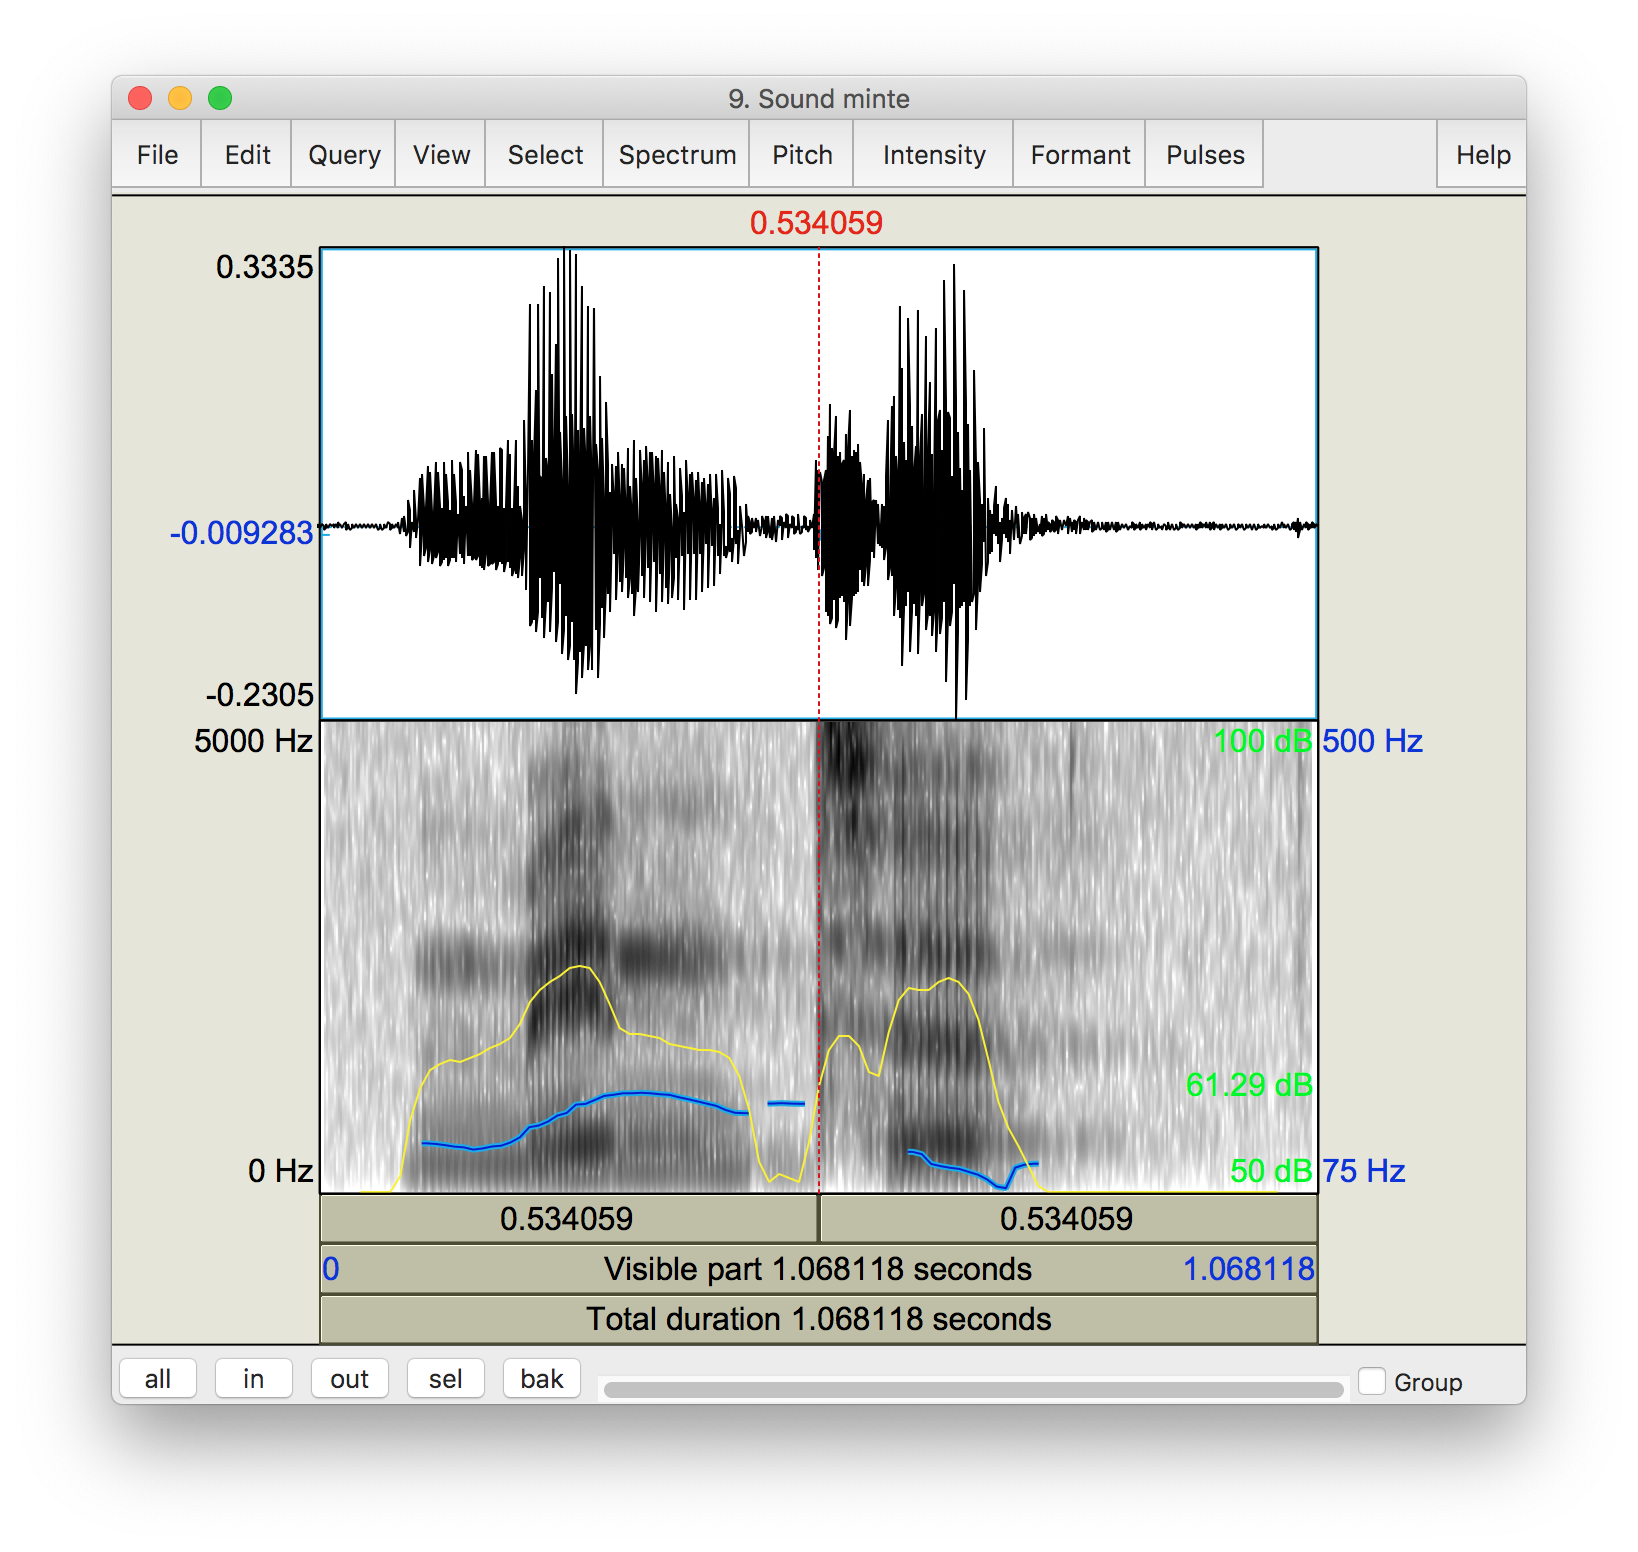
\includegraphics[height=0.8\textheight]{images/minte}
\end{frame}

\begin{frame}
  {Drucksilben und Schallsilben (Sievers, siehe \citealt{Maas2002})}
  \Large
  \textit{Miete}\\
  \Zeile
  \centering
  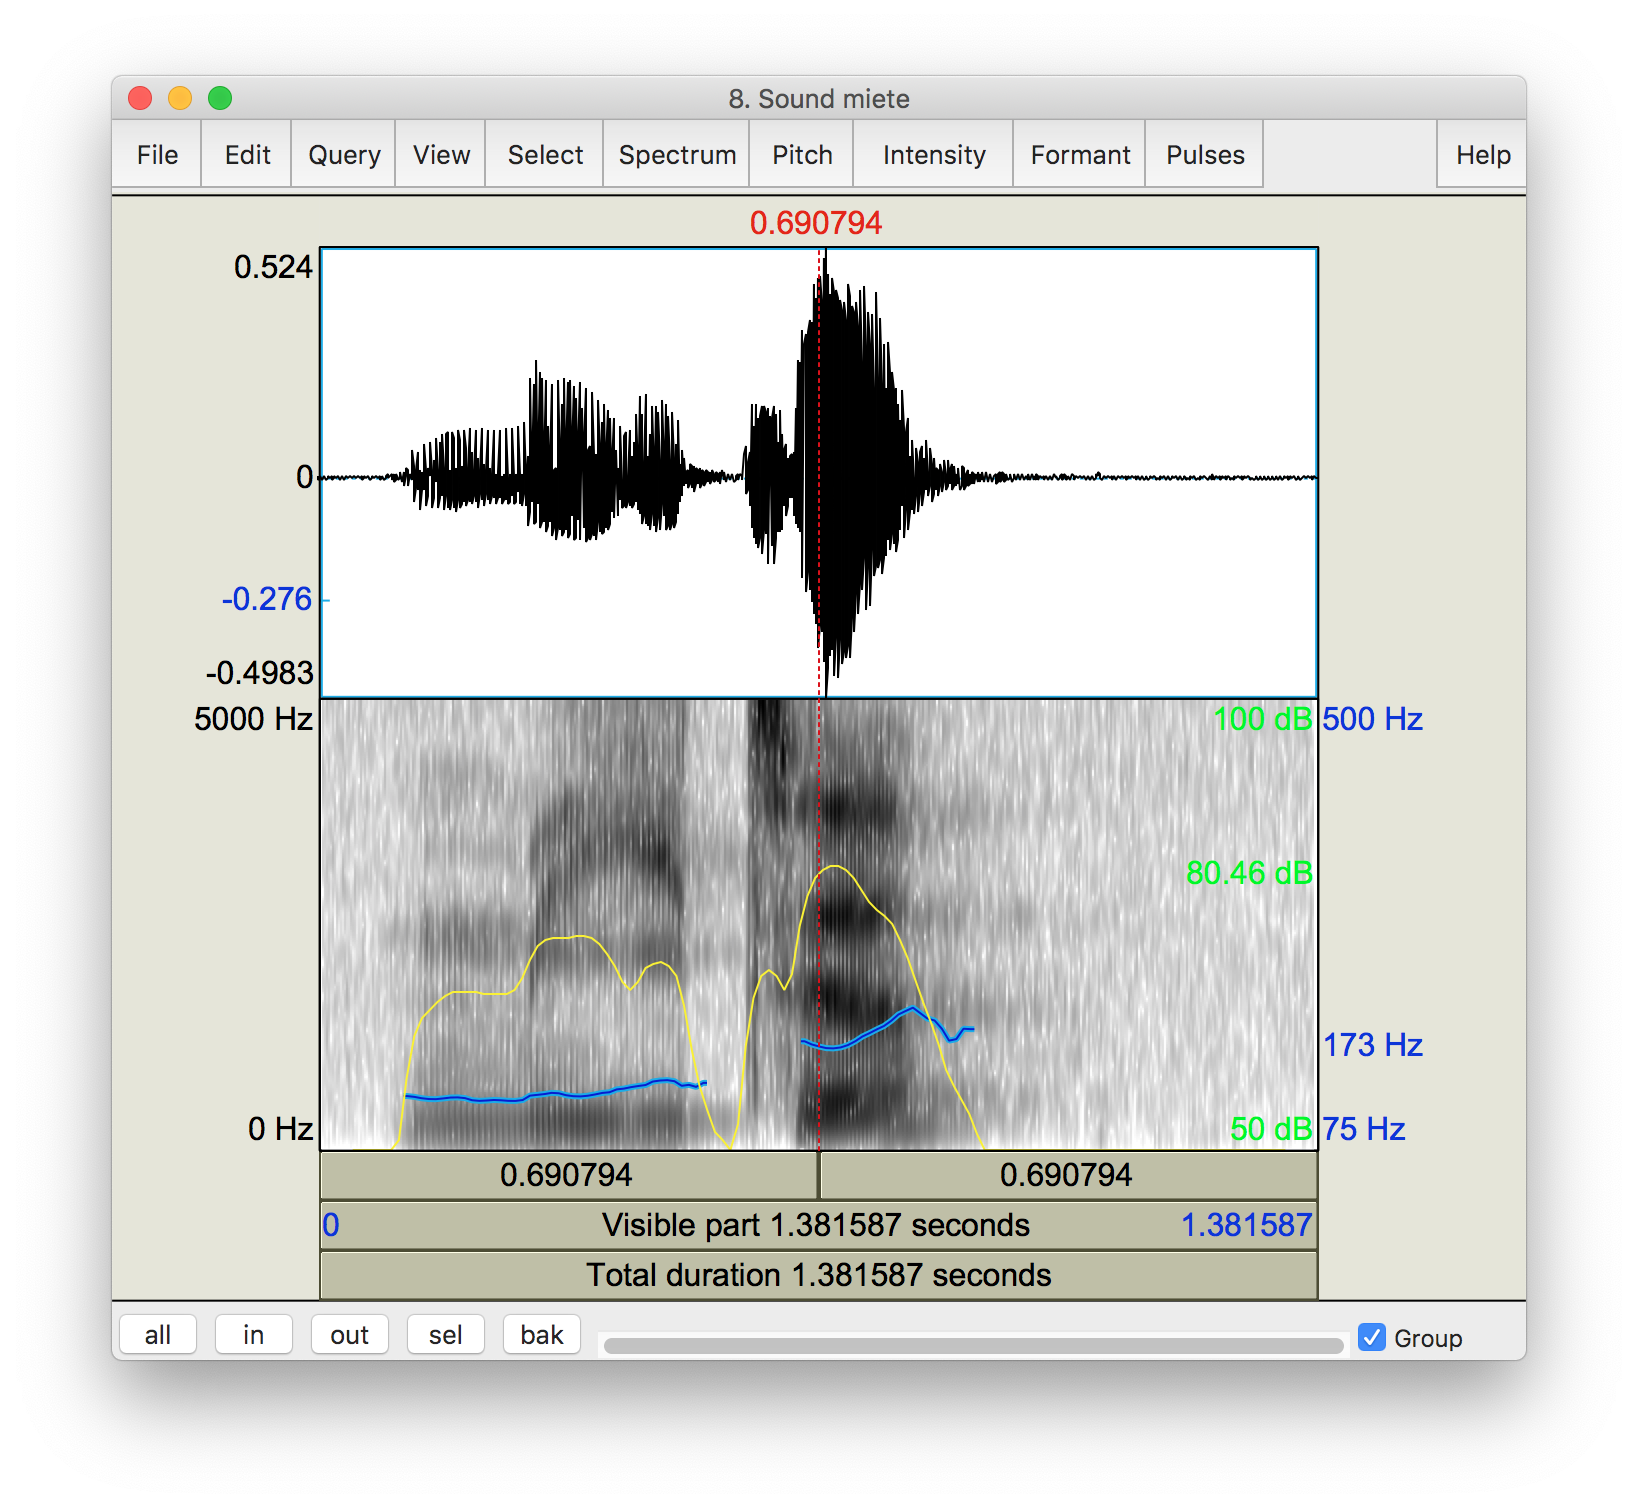
\includegraphics[height=0.8\textheight]{images/miete}
\end{frame}

\begin{frame}
  {Drucksilben und Schallsilben (Sievers, siehe \citealt{Maas2002})}
  \Large
  \textit{Mitte}\\
  \Zeile
  \centering
  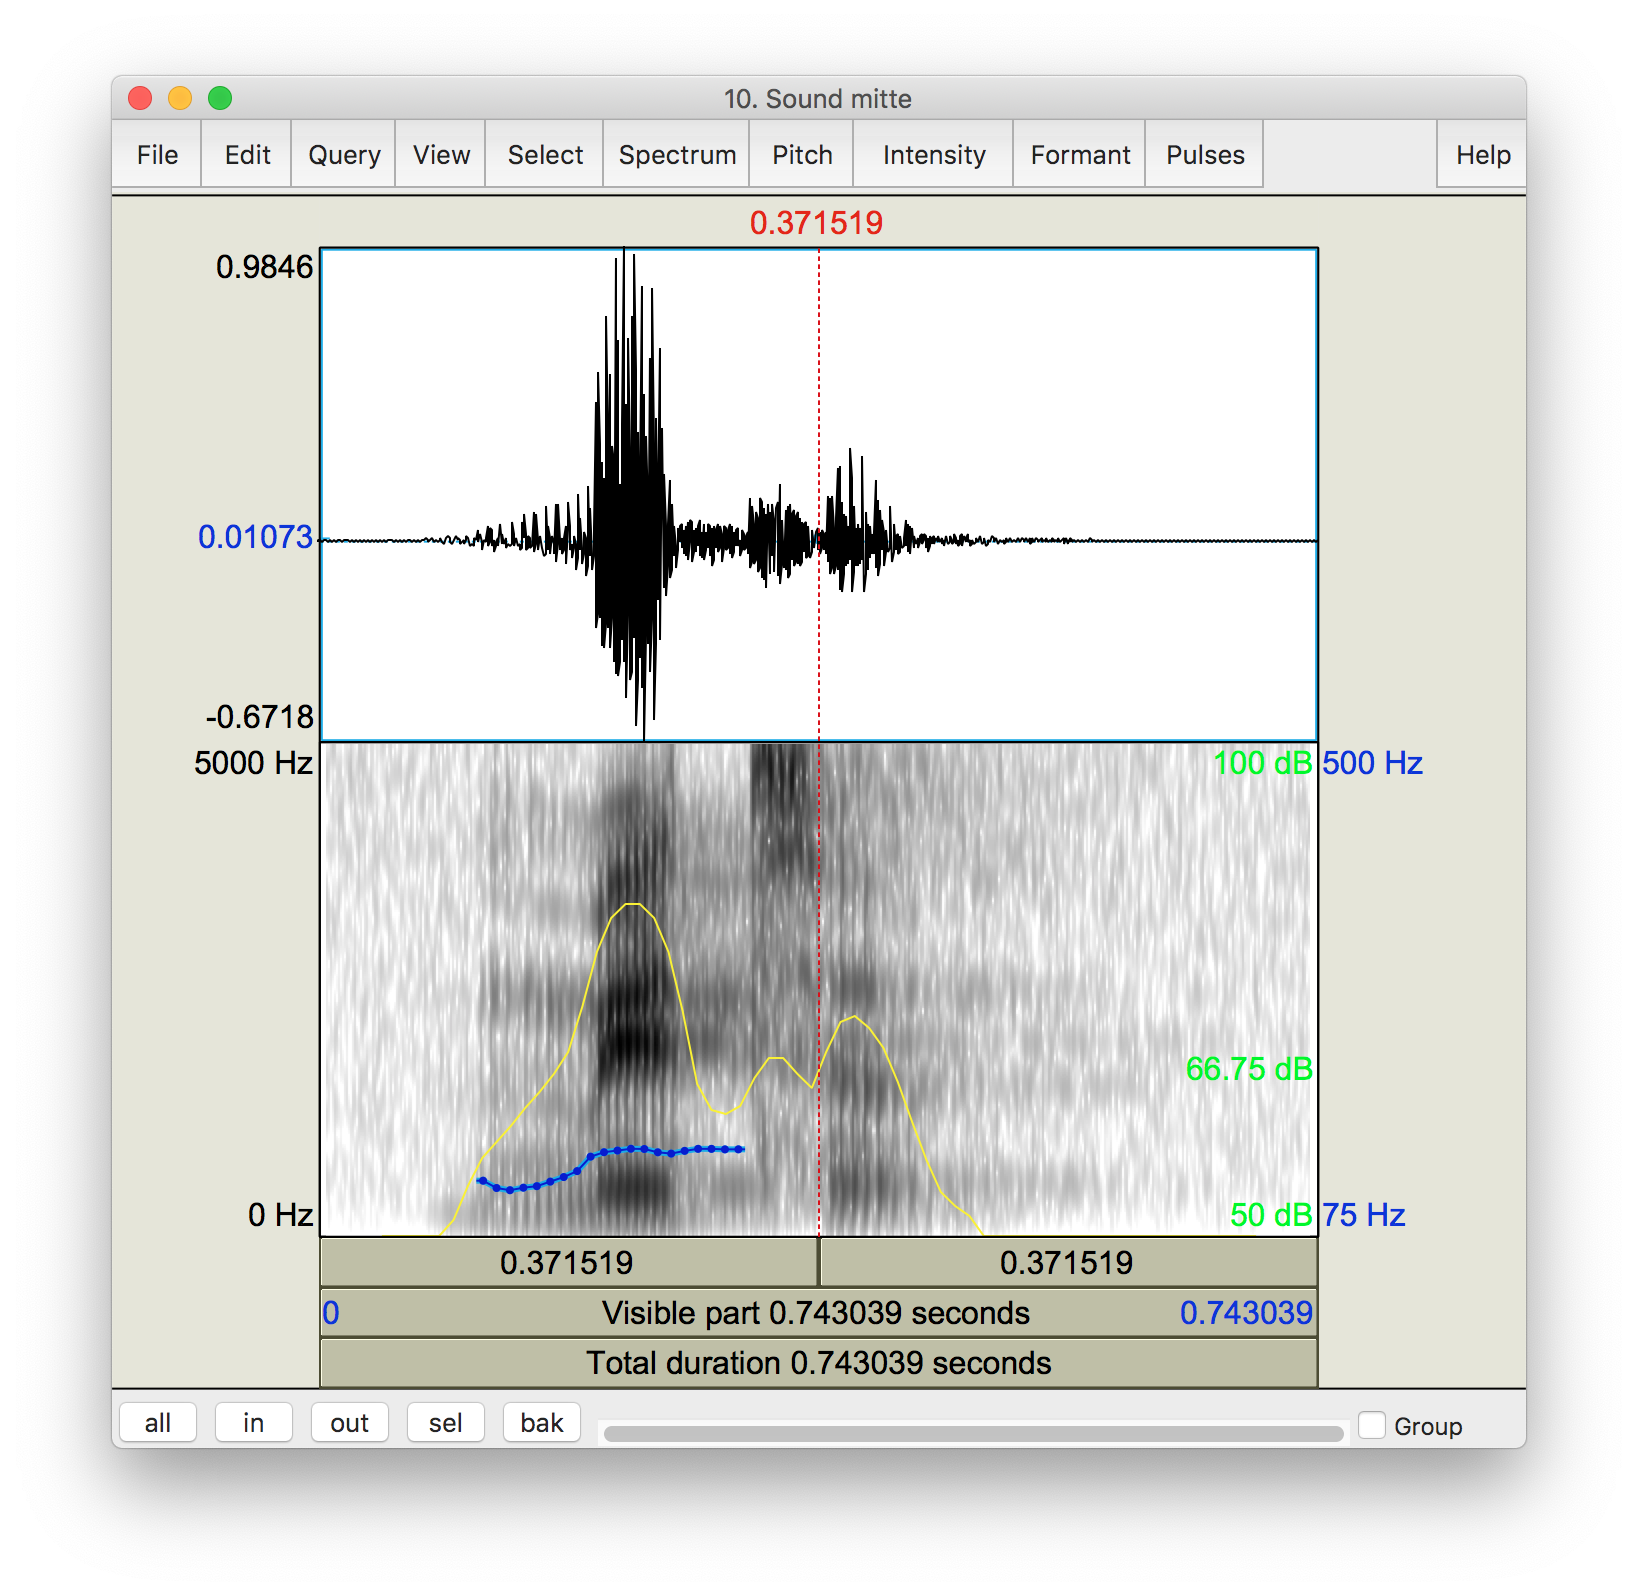
\includegraphics[height=0.8\textheight]{images/mitte}
\end{frame}

\begin{frame}
  {Maximierung des Anfangsrands}
  \pause
  Es bleiben immer noch Zweifelsfälle bei der wortinternen Silbifizierung\dots\\
  \pause
  \Zeile
  \begin{exe}
    \ex\textit{freches} \alert{[fʁɛç̣əs]}, \rot{*[fʁɛç.əs]}
    \pause
    \ex\textit{komplett} \alert{[kɔm.plɛt]}, \rot{*[kɔmp.lɛt]}
    \pause
    \ex\textit{Betreff} \alert{[bə.tʁɛf]}, \rot{*[bət.ʁɛf]}
  \end{exe}
  \Zeile
  \pause
  \Large
  Strukturbedingung: So viele Konsonanten wie möglich\\
  in den \alert{Anfangsrand} statt in den Endrand.\\
  \Zeile
  \pause
  \normalsize
  Und denken Sie schonmal über \alert{morphologische Beschränkungen} auf Silbifizierung nach.
  Vielleicht kommen wir in der Morphologie darauf zurück.
\end{frame}


\begin{frame}
  {Die Klatschmethode und die Hinhörschreibung}
  \pause
  "`Hinhörschreibungen"'?\\
  \begin{itemize}[<+->]
    \item E\rot{h}e, we\rot{h}e
    \item Ra\rot{d}, Wan\rot{d}, Bun\rot{d}
    \item bri\rot{ng}, Go\rot{ng}
    \item Köni\rot{g}, weni\rot{g}, wichti\rot{g}
    \item \rot{S}tein, \rot{S}palte
  \end{itemize}
  \pause
  "`Klatschmethode"'?\\
  \begin{itemize}[<+->]
    \item Krie\rot{ch}er, rö\rot{tl}ich, Nö\rot{rgl}er, a\rot{bsp}a\rot{lt}en, Ä\rot{rzt}e, plö\rot{tzl}ich
    \item rate, ratte
    \item Matsche
    \item Küche
    \item bringe
  \end{itemize}
\end{frame}


\begin{frame}
  {Und wie geht es richtig?}
  \Zeile
  \large
  Denken Sie bitte bis zur nächsten Woche darüber nach, wie sie Silbenstruktur im schulischen Bereich vermitteln würden!
  Wichtige Punkte sind zum Beispiel:\\
  \Zeile
  \begin{itemize}
    \item Was ist die \alert{Fähigkeit}, die vermittelt werden soll?
    \item Welches \alert{Wissen} ist nötig, um diese zu erwerben?
    \item Welchen \alert{Übungs-Input} müssen Sie den Lernenden geben?
    \item Wie stellen Sie diesen Input zusammen\\
      (\alert{Form und Gruppierung des Inputs})?
  \end{itemize}
%   \begin{itemize}[<+->]
%     \item eigentlich nicht meine Aufgabe, aber\dots
%       \Zeile
%     \item \alert{Bewusstsein für Länge}
%     \item Bewusstsein für \alert{Länge je nach Position}
%     \item kurz vor Vokal im Wort $\Rightarrow$ Silbengelenk, Gelenkschreibung
%       \Zeile
%     \item \rot{Formenreihen als Ausgangsbasis}, \alert{nur Kernwortschatz}
%     \item Anfang mit dem \alert{Einsilbler} (ohne Dehnungsschreibung?)
%     \item weiter mit dem \alert{trochäischen Zweisilbler ohne Silbengelenk}
%     \item schließlich \alert{Zweisilbler mit Silbengelenk}
%     \item für Anfangsrandmaximierung: Parallele zum \alert{Einsilbler}
%   \end{itemize}
\end{frame}

\section{Vorschau}

\begin{frame}
  {Nächste Woche: Wortklassen und Wortarten}
  \pause
  \begin{itemize}[<+->]
    \item Was sind Wörter?
    \item Sind Wortklassen durch \alert{Bedeutungen} definiert?
    \item \alert{morphologische} Definitionen von Wortklassen
    \item \alert{syntaktische} Definitionen von Wortklassen
    \item \alert{Wie viele Wortklassen gibt es?}
  \end{itemize}
  \pause
  \Zeile
  \centering
  \Large
  \alert{Bitte lesen: Kapitel 6 komplett,\\
  mindestens aber 6.2 (S.~174--191)}
  \pause
  \pause
  \pause
  \pause
  \pause
\end{frame}


\begin{frame}
  {Literatur}
  \renewcommand*{\bibfont}{\footnotesize}
  \setbeamertemplate{bibliography item}{}
  \printbibliography
\end{frame}

\end{document}
